\documentclass[12pt]{article}
\usepackage[margin=1in]{geometry}
\usepackage[T1]{fontenc}
\usepackage[USenglish]{babel}
\usepackage[nodayofweek,level]{datetime}
\usepackage{amsfonts}
\usepackage{amsmath}
\usepackage{amssymb}
\usepackage{tikz}
\usetikzlibrary{intersections,arrows.meta}
\usepackage{pgfplots}
\usepackage[scr]{rsfso}
\usepackage{array}

\usepackage{tikz,pgfplots}

\pgfplotsset{compat=1.10}
\usepgfplotslibrary{fillbetween}
% Change due date below
\newcommand{\dueDate}{\formatdate{13}{10}{2017}}

\begin{document}
	
%\selectlanguage{USenglish}	

\title{Homework: Week 2}
\author{Joseph Ismailyan}
\date{}
\maketitle
\begin{flushleft}
Math 100 \\
Due: \dueDate \\ 
Professor Boltje \\
MWF 9:20a-10:25a
\end{flushleft}

% Insert first section here
% Minipage creates the columns
\begin{minipage}[t]{0.40\textwidth}
\section*{Section 1.6}

\subsection*{6.}
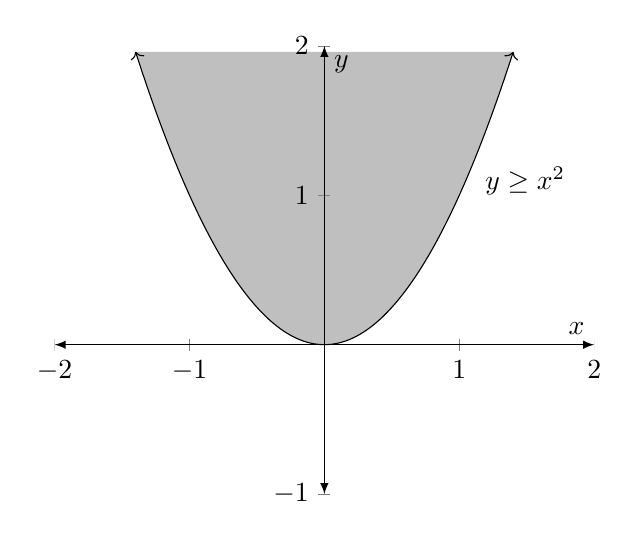
\begin{tikzpicture}
\begin{axis}[
xmin=-2, xmax=2,
ymin=-1, ymax=2,
axis lines=center,
axis on top=true,
domain=0:1,
xlabel={$x$},
ylabel={$y$},
axis line style={latex-latex}
]
\addplot [
name path=A,
domain=-1.4:1.4,
samples=100, 
color=black,
%dashed,
<->,
] 
{x^2}
node [pos=0.85, below right]{$ y\geq x^2 $};
\addplot [name path=B,opacity=0,domain=-1.4:1.4] {1.96};
\addplot[gray!50] fill between[of=A and B];
\end{axis}
\end{tikzpicture}
\bigskip

\end{minipage}
% Creates verticle line
\hfill\vline\hfill
\begin{minipage}[t]{0.45\textwidth}



\section*{Section 1.7}

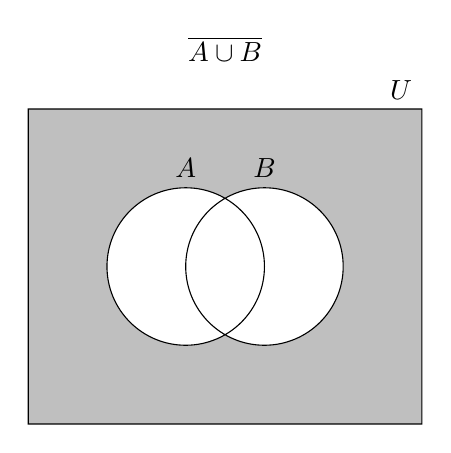
\begin{tikzpicture}[fill=gray!50]
% outline
\fill (-2,-2) rectangle (3,2);
\fill[white] (0,0) circle (1);
\fill[white] (1,0) circle (1);
\draw (0,0) circle (1) (0,1)  node [text=black,above] {$A$}
(1,0) circle (1) (1,1)  node [text=black,above] {$B$}
(-2,-2) rectangle (3,2) node [text=black,above left] {$U$};
\node[anchor=south] at (current bounding box.north) {$ \overline{A \cup B}$};
\end{tikzpicture}

\bigskip

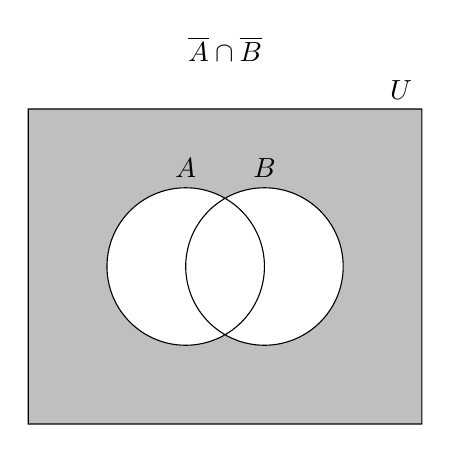
\begin{tikzpicture}[fill=gray!50]
% outline
\fill (-2,-2) rectangle (3,2);
\fill[white] (0,0) circle (1);
\fill[white] (1,0) circle (1);
\draw (0,0) circle (1) (0,1)  node [text=black,above] {$A$}
(1,0) circle (1) (1,1)  node [text=black,above] {$B$}
(-2,-2) rectangle (3,2) node [text=black,above left] {$U$};
\node[anchor=south] at (current bounding box.north) {$\overline{A} \cap \overline{B}$};
\end{tikzpicture}
\\

Answer: From the two diagrams above, we can see that the sets are equal.
\end{minipage}
\pagebreak


\begin{minipage}[t]{0.40\textwidth}
	\section*{Section 1.8}
\subsection*{6(a).}
Answer:
$\bigcup\limits_{ i \in \mathbb{N}}[0,i+1]=[0,\infty)$


\subsection*{6(b).}
Answer:
$\bigcap\limits_{ i \in \mathbb{N}}[0,i+1]=[0,2]$

\section*{Section 2.1}
\subsection*{6.}
Question: Some sets are finite.
\\\\
Answer: It is statement because it can be proven definitely true or false.


\subsection*{14.}
Question: Call me Ishmael.
\\\\
Answer: It is a sentence because it isn't a mathematical expression. 

\section*{Section 2.2}
\subsection*{8.}
Question: At least one of the 
numbers $ x $ and $ y $ equals $ 0 $.
\\
$ P: x $ is equal to 0.\\
$ Q: x $ is equal to 0.\\\\
Answer: $ P\lor Q $

\end{minipage}
% Creates verticle line
\hfill\vline\hfill
\begin{minipage}[t]{0.45\textwidth}
\section*{Section 2.3}
\subsection*{2.}
Problem: Convert the following sentences to be in the form $ P \implies Q $
$ P: $ A function is differentiable.\\
$ Q: $ A function is continuous.\\\\
Answer: $ P \implies Q $
\section*{Section 2.4}
\subsection*{4.}
Problem: Convert to the form "$ P $ if and only if $ Q $". \\
$ P: a \in \mathbb{Q}$\\
$ Q: 5a \in \mathbb{Q}$\\\\
Answer: $ P \Leftrightarrow Q $\\
$ a \in \mathbb{Q} $ if and only if $ 5a \in \mathbb{Q} $

\section*{Section 2.5}
\subsection*{4.}
Problem: Write a truth table for the logical problem: 
$ \sim (P \lor Q) \lor \sim(P) $\\
\[
\begin{array}{c|c|c|c|c}
P & Q &  \sim(P \lor Q) &  \sim(P)  & \sim(P \lor Q) \lor \sim(P)\\
\hline
T & T & F & F & F\\
T & F & F & F & F\\
F & T & F & T & T\\
F & F & T & T & T
\end{array}
\]


\end{minipage}
\pagebreak


\begin{minipage}[t]{0.40\textwidth}
\section*{Section 2.5 cont.}
\subsection*{8.}
Problem: Write a truth table for the logical problem: 
$ P \lor (Q \lor \sim R)$\\
\[
\begin{array}{c|c|c|c|c}
P & Q & R &(Q \lor \sim R) & P \lor (Q \lor \sim R)\\
\hline
T & T & T & T & T\\
T & T & F & T & T\\
T & F & T & F & T\\
T & F & F & T & T\\
F & T & T & T & T\\
F & T & F & T & T\\
F & F & T & F & F\\
F & F & F & T & T
\end{array}
\]

\subsection*{10.}
Problem: Suppose the statement $ ((P \land Q) \lor R) \implies (R \lor S)$\\
is false. Find the truth values of $ P,Q,R $ and $ S. $\\\\
Asnwer: Suppose $ A $ and $ B $ are statements. The only way that $(A \implies B)=False$ is if $ A=True $ and $ B=False $. Therefore $ ((P \land Q) \lor R)$ must be $ True $ and $ (R \lor S) $ must be $ False $. For $ (R \lor S) $ to be $ False $, both $ R $ and $ S $ must be $ False $. Since $ R $ is false, the statement $ (P \land Q) \lor R) $ relies on $ (P \land Q) $ to be true so both $ P $ and $ Q $ must be true. In conclusion: 
$$
\begin{array}{c|c|c|c}
	P & Q & R & S\\
	\hline
	T & T & F & F\\
\end{array}
$$

\end{minipage}
% Creates verticle line
\hfill\vline\hfill
\begin{minipage}[t]{0.45\textwidth}
\section*{Section 2.6}
\subsection*{2.}
Problem: Show that the following statements are logically equivalent.\\
$ a $: $ P \lor (Q \land R) $\\
$ b $: $ (P \lor Q) \land (P \lor R) $ \\
\[
\begin{array}{c|c|c|c|c}
P & Q & R &(Q \land R) & P \lor (Q \land R)\\
\hline
T & T & T & T & T\\
T & T & F & F & T\\
T & F & T & F & T\\
T & F & F & F & T\\
F & T & T & T & T\\
F & T & F & F & F\\
F & F & T & F & F\\
F & F & F & F & F
\end{array}
\]
\[
\begin{array}{c|c|c|c|c|c}
P & Q & R &(P \lor Q) & (P \lor R) & (P \lor Q) \land (P \lor R)\\
\hline
T & T & T & T & T & T\\
T & T & F & T & T & T\\
T & F & T & T & T & T\\
T & F & F & T & T & T\\
F & T & T & T & T & T\\
F & T & F & T & F & F\\
F & F & T & F & T & F\\
F & F & F & F & F & F
\end{array}
\]
\subsection*{10.}
Decide whether the following statements are logically equivalent:\\
$ a.\quad(P \implies Q) \lor R $\\
$ b. \sim((P \land \sim Q) \land \sim R) $\\
$1) \quad (P \implies Q) \lor R $ = $ (\sim P \lor Q) \lor R$ \\by definition of implication\\
$ 2) \quad (\sim P \lor Q) \lor R =  \enspace \sim((\sim P \lor Q) \lor R)$\\
by DeMorgan's Laws\\
$ 3) \sim((\sim P \lor Q) \lor R) = \sim(\sim P \lor Q) \land \sim R $\\
by DeMorgan's Laws\\
$ 4) \sim(\sim P \lor Q) \land \sim R = (P \land \sim Q) \land \sim R$\\
by DeMorgan's Laws\\
$ 5)\quad (P \land \sim Q) \land \sim R =\\ \sim ((P \land \sim Q) \land \sim R) = b$\\\\
$\therefore a \equiv b $, they're logically equivalent.
\end{minipage}









\end{document}